\section{Methods}\label{art.meth}
This section briefly reviews the transmission model used,
and outlines the analyses conducted to answer the research questions outlined above.
%===================================================================================================
\subsection{Model}\label{art.meth.model}
The complete details of model structure, parameterization, and calibration
are given in Chaper~\ref{model}.
The proposed force of infection approach from in Chapter~\ref{foi} was used throughout.
Briefly, the deterministic compartmental model features
8 risk groups, including higher and lower risk FSW and clients, and
4 partnership types, including regular and occasional sex work (Figure~\ref{fig:model.risk}).
Risk heterogeneity is captured through group-level factors, including
group sizes, turnover, GUD prevalence, and different numbers/types of partnerships;
as well as partnership-level factors, including
mixing patterns, partnership durations, frequency of vaginal and anal sex, and levels of condom use.
Modelled HIV natural history includes acute infection and stages defined by CD4 count, which
determine differences in infectiousness, HIV-attributable mortality, and historical ART eligibility.
I obtained $N_f = 1000$ plausible model fits via calibration.
%===================================================================================================
\subsection{Scenarios \& Analyses}\label{art.meth.obj}
%---------------------------------------------------------------------------------------------------
\subsubsection{Objective 1: Influence of cascade differences between risk groups}\label{art.meth.obj.1}
For Objective~\ref{obj:art.1},
I defined the \emph{base case} scenario to reflect
observed cascade scale-up in Eswatini, reaching \cashi by 2020 \cite{AIDSinfo}.
Next, I defined 4 \emph{counterfactual} scenarios in which overall viral suppression was lower,
such that the population overall reached \casmd by 2020,
reflecting approximate trends in SSA cascades prior to universal ART \cite{AIDSinfo}.
In these counterfactual scenarios, I reduced cascade progression
among specific risk groups in different combinations:
FSW, clients, and/or the remaining population (``lower risk'').
I reduced cascade progression by calibrating and applying
a constant relative scaling factor ``$R$'' to group-specific rates of:
diagnosis ($R_d \in [0,1]$),
treatment initiation ($R_t \in [0,1]$), and
treatment failure / discontinuation ($R_u \in [1,20]$).
When FSW and/or clients had reduced cascade, I calibrated their $R$s so that
these populations achieved approximately \caslo by 2020.
By contrast, I calibrated $R$s for the lower risk population so that
the Swati population \emph{overall} achieved \casmd in all 4 counterfactual scenarios,
thus ensuring that a consistent proportion of the population overall
experienced reduced viral suppression.
Table~\ref{tab:art.scenarios} summarizes these scenarios, while
Figure~\ref{fig:art.1.cascade} plots the modelled cascades over time.
When cascade rates among FSW and/or clients were unchanged from the base case,
the cascade these groups achieved could be lower than \cashi
due to risk group turnover and higher incidence.
All cascades continued to increase beyond 2020 due to assumed fixed rates of
diagnosis, treatment initiation, and treatment failure / discontinuation thereafter.
\begin{table}
  \centering
  \caption{Modelling scenarios for Objective~\ref{obj:art.1} defined by 2020 calibration targets}
  \label{tab:art.scenarios}
  \begin{tabular}{lcccccc}
  \toprule
  & \multicolumn{3}{c}{ART cascade in 2020\tn{a}}
  & \multicolumn{3}{c}{Re-scaled cascade rates\tn{b}} \\
  \cmidrule(rl){2-4}\cmidrule(rl){5-7}
  Scenario & FSW & Clients & Overall & FSW & Clients & Lower Risk \\
  \midrule
  \emph{Base Case}                    & \cashi &   ---  & \cashi &  --- &  --- &  --- \\
  \emph{Leave Behind: FSW}            & \caslo &   ---  & \casmd & \yes & \no  & \yes \\
  \emph{Leave Behind: Clients}        &   ---  & \caslo & \casmd & \no  & \yes & \yes \\
  \emph{Leave Behind: FSW \& Clients} & \caslo & \caslo & \casmd & \yes & \yes & \yes \\
  \emph{Leave Behind: Neither}        &   ---  &   ---  & \casmd & \no  & \no  & \yes \\
  \bottomrule
\end{tabular}
\floatfoot{
  \tnt[a]{Cascade: \% diagnosed among PLHIV; \% on ART among diagnosed; \% virally suppressed among on ART};
  \tnt[b]{Rates of: diagnosis; ART initiation; treatment failure};
  \ffpopz.
  Figure~\ref{fig:art.1.cascade} plots the modelled cascades over time.}

\end{table}
\par
I quantified ART prevention impacts via relative
cumulative additional infections (CAI) and additional incidence rate (AIR)
in the counterfactual scenarios ($k$) \vs the base case ($0$),
over multiple time horizons up to 2030, starting from $t_0 = 2000$:
\begin{equation}
  \txn{CAI, AIR}\,(t) = \frac{\Omega_{k}(t) - \Omega_{0}(t)}{\Omega_{0}(t)}
  ,\qquad \Omega(t) =
  \begin{cases}
    ~\int_{t_0}^{t}\!\Lambda(\tau)\,d\tau & \txn{CAI} \\
    ~\lambda(t) & \txn{AIR}
  \end{cases}
\end{equation} where:
$\Lambda$ denotes absolute numbers of infections per year, and
$\lambda$ denotes incidence rate per susceptible per year.
For each scenario, I computed these outcomes (CAI and AIR) for each model fit $j$,
and reported median (95\% CI) values across model fits, reflecting uncertainty.
%---------------------------------------------------------------------------------------------------
\subsubsection{Objective 2: Conditions under which cascade differences matter most}\label{art.meth.obj.2}
For Objective~\ref{obj:art.2}, I estimated via regression:
the effects of lower cascade among certain risk groups on relative CAI and AIR,
plus potential effect modification by epidemic conditions.
The hypothesized causal effets are illustrated
as a directed acyclic graph in Figure~\ref{fig:art.2.dag},
and the synthetic data generation processes and variable definitions are as follows.
\par
For this regression analysis, I obtained 10,000 samples.
I explored a wider range of counterfactual scenarios \vs Objective~\ref{obj:art.1}
by randomly sampling the relative rates for
diagnosis and treatment initiation $R_d, R_t \sim \opname{Beta}(\alpha=3.5,\beta=1.9)$
and treatment failure $R_u \sim \opname{Gamma}(\alpha=3.4,\beta=1.9)$
for each of: FSW, clients, and the remaining lower risk population (9~total values).
These sampling distributions had 95\%~CI: (0.25,~0.95) and (1.5,~15), respectively,
and were chosen to obtain cascades in 2020 spanning
approximately \mbox{60-60-90} through \mbox{90-90-95} (Figure~\ref{fig:art.2.cascade}). % MAN
For each of $N_f = 1000$ model fits, I generated $N_k = 10$ counterfactual scenarios per fit
via random relative rates ``$R$'' via Latin hypercube sampling,
yielding $N_f N_k = {}$10,000 total counterfactual samples for the regression.
\begin{figure}
  \centering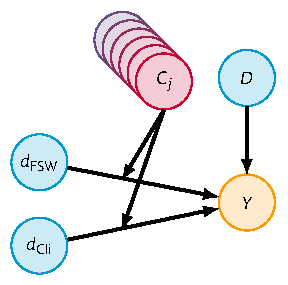
\includegraphics[scale=1]{art.2.dag}
  \caption{Directed acyclic graph (DAG) for inferring
    the epidemic conditions under which
    differential viral suppression across risk groups matters most}
  \label{fig:art.2.dag}
  \floatfoot{
    $Y$: cumulative additional infections (CAI) or additional incidence rate (AIR) by 2030;
    $D$: difference in population-overall viral unsuppression
      in counterfactual \vs base case scenario;
    $d_i$: difference in group-$i$-specific viral unsuppression
      \vs population overall within counterfactual scenario;
    $C_j$: epidemic conditions (effect modifiers of $d_i$).}
\end{figure}
\par
For each of these 10,000 samples, I defined
relative CAI and AIR by 2030 \vs the base case, as in Objective~\ref{obj:art.1}.
For each sample, I further defined
$U_{fki}$ for risk groups $i \in \{\tdef{1}{FSW}, \tdef{2}{clients}, \tdef{*}{overall}\}$
as the proportions virally unsuppressed among people living with HIV by 2020,
reflecting a summary measure of ART cascade gaps.
Using $U_{fki}$, I defined the main regression predictors as:
$D_{fk} = U_{fk*} - U_{f0*} > 0$, reflecting differences in
\emph{population-overall} viral unsuppression in sample $k \in [1,10]$
\vs the base case (denoted $k = 0$); and
$d_{fki} = U_{fki} - U_{fk*} \lessgtr 0$, reflecting differences in
\emph{group-$i$-specific} viral unsuppression in sample $k$
\vs the population overall in sample $k$ --- \ie disproportionate unsuppression.
\par
Next, I defined the following measures of epidemic conditions ($C_{fj}$) related to sex work,
as hypothesized modifiers of the effect of disproportionate unsuppression on relative CAI and RAI:
FSW and client population sizes (\% of population overall);
average rate of turnover among FSW and clients
(per year, reciprocal of duration selling / buying sex); and
HIV incidence ratios in the year 2000 among FSW \vs other women, and among clients \vs other men.
For these measures, I combined higher and lower risk FSW,
and likewise higher and lower risk clients.
I used HIV incidence ratios in 2000 to reflect
summary measures of risk heterogeneity prior to ART,
as compared to including all modelled risk factors
for HIV acquisition (\eg Table~\ref{tab:sr.factors}),
which could lead to overfitting and improper inference due to effect mediation. % TODO: collinearity?
\par
Finally, I defined a general linear model for each outcome (CAI, AIR) as:
\begin{equation}\label{eq:art.glm}
  \txn{CAI, AIR} = \beta_0\,D
                 + \sum_i \beta_i\,d_i
                 + \sum_{ij} \beta_{ij}\,d_i\,C_j
\end{equation}
such that each outcome is modelled as a sum of the effects of:
differential population-level unsuppression in the counterfactual
\vs the base scenario ($D$);
differential unsuppression among FSW and clients
\vs the population overall within the counterfactual scenario ($d_i$); and
effect modification of $d_i$ by epidemic conditions ($C_j$).
The model does not include an intercept because if $D = d_i = 0$,
then we expect $\txn{CAI} = \txn{AIR} = 0$.
I fitted this model for each outcome using generalized estimating equations \cite{Halekoh2006}
to control for repeated use of each model fit $f$.
I standardized all model variables ($D$, $d_i$, $C_j$) via
$\hat{x} = (x - \txn{mean}(x)) / \txn{SD}(x)$
to avoid issues of different variable scales and collinearity in interaction terms.
This standardization does not imply that
regression coefficient magnitudes can be compared to indicate variable ``importance'',
because the standardization applied to each variable is driven
by the variance before standardization
--- in this case reflecting arbitrary ranges ($D$, $d_i$) or uncertainty in calibration ($C_j$).%
\footnote{I verified that results were qualitatively the same using
  $\hat{x} = (x - \txn{median}(x)) / \txn{IQR}(x)$.
  For further discussion on interpretation of standardized regression coefficients,
  see also: \hreftt{stats.stackexchange.com/questions/29781} and links therein.}
Rather, effect sizes can be interpreted as:
the expected change in outcome per standard deviation change in the variable.
